\documentclass[letterpaper]{article}
% \usepackage{fontspec}

% ==================================================

% document parameters
% \usepackage[spanish, mexico, es-lcroman]{babel}
\usepackage[spanish]{babel}
\usepackage[margin = 1in]{geometry}
\decimalpoint

% ==================================================

% Packages for math
\usepackage{mathrsfs}
\usepackage{amsfonts}
\usepackage{amsmath}
\usepackage{amsthm}
\usepackage{amssymb}
\usepackage{physics}
\usepackage{dsfont}
\usepackage{esint}

% ==================================================

% Packages for writing
\usepackage{enumerate}
\usepackage[shortlabels]{enumitem}
\usepackage{framed}
\usepackage{csquotes}

% ==================================================

% Miscellaneous packages
\usepackage{siunitx}        % Para colocar unidades según SI.  Ej \unit{\centi\meter}
\usepackage{float}
\usepackage{tabularx}
\usepackage{xcolor}
\usepackage{multicol}
\usepackage{subcaption}
\usepackage{caption}
\captionsetup{format = hang, margin = 10pt, font = small, labelfont = bf}

% Citation
\usepackage[round, authoryear]{natbib}

% Hyperlinks setup
\usepackage{hyperref}
\definecolor{links}{rgb}{0.36,0.54,0.66}
\hypersetup{
   colorlinks = true,
    linkcolor = black,
     urlcolor = blue,
    citecolor = blue,
    filecolor = blue,
    pdfauthor = {Author},
     pdftitle = {Title},
   pdfsubject = {subject},
  pdfkeywords = {one, two},
  pdfproducer = {LaTeX},
   pdfcreator = {pdfLaTeX},
   }

\input{format}
\input{commands}

\begin{document}

\begin{Large}
    \textsf{\textbf{Práctica 4. Microscopio}}
\end{Large}

\vspace{1ex}

\textsf{\textbf{Estudiante:}} \\
\text{Andrés Felipe Pinzón Harker}, \href{mailto:apinzonh@unal.edu.co}{\texttt{apinzonh@unal.edu.co}}\\
\text{Cristian}, \href{mailto:al@unal.edu.co}{\texttt{crisxd@unal.edu.co}}\\
\textsf{\textbf{Profesor:}} \text{Omar Olarte Duarte}

\vspace{2ex}

\section*{TO DO (BORRAR ANTES DE ENVIAR)}
\subsection*{Necesarios}
\begin{itemize}
    \item Hallar el aumento nominal del microscopio. Indicar que el realmente importante es el objetivo, el ocular no sirve pa nah supuestamente
    \item Indicar dónde quedan ubicadas las pupilas de entrada y salida resolviendo (creo) teóricamente el esquema.
    \item Ignorar el 4.
    \item Indicar el efecto de la modificación de distancia de la pupila en el experimento.
    \item Dar los resultados al respecto de las pupilas ubicadas y comparaciones.
\end{itemize}
\subsection*{Posibles}
\begin{itemize}
    \item Indicar la resolución del microscopio.
    \item Incluir un esquema ilustrativo del real experimento
\end{itemize}

\section*{\textsf{Introducción}}

En esta práctica experimental, se responde la cuestionario 4 de la clase \textit{Mediciones en Óptica y Acústica} del semestre 2024-II del Departamento de Física de la Universidad Nacional de Colombia, con la finalidad de dar claridad del funcionamiento del sistema óptico del \textbf{microscopio} en conformación de lentes convergentes (objetivo y ocular) con focos conocidos $f_1$ y $f_2$.

\section*{\textsf{Modelación Teórica}}

Se conformó el esquema del Microscopio sin acomodación (véase fig. \ref{fig:esquema}), buscando con ello las ventajas proveídas como: no acomodar la mirada para tener la imagen aumentada, brinda una imagen nítida y clara a distancias fijas, principalmente; restar la importancia de la observación en el lente ocular (\textit{OC}), brindando ventajas en el cambio del lente objetivo (\textit{OB}) sin necesidad de re acomodación del ocular; tener medidas precisas reglamentarias según normativas vigentes, en nuestro caso se siguió norma DIN (largo de tubo $l_t = 160 \, \unit{\milli \meter}$).
\begin{figure}[H]
    \centering
    
\includegraphics[width=0.8\linewidth]{figs/esquema_notgrid.png}
    \caption{Esquema experimental del microscopio, donde se requiere que la imagen $s_i^{\prime}$ se acomode en el foco primario del ocular $f_2$ para tener la vista sin acomodación.}
    \label{fig:esquema}
\end{figure}

Las desventajas hacen parte del objeto de estudio: aberraciones producto del lente, variaciones con el diafragma en el estudio del ``enfoque'' de la pupila (pupila de salida $P_{ex}$ y de entrada $P_{en}$) de la imagen, y la nitidez producto de la colocación.

Se conoce de este esquema lo siguiente: el \textit{OB} será el diafragma de apertura (\textit{DA}) siempre que no haya un elemento físico inserto; la pupila de salida estará a la derecha del ocular formando una imagen real de menor tamaño que el \textit{DA}.

El \textit{aumento nominal} está dado (\cite{Yobani_Optica2020}), según las especificaciones dadas anteriormente de este microscopio, como:
\begin{equation}
    m = M_{OC} M_{OB} = -\frac{l_t}{f_{OB}}\frac{250}{f_{OC}}
    \label{eq:aumento_nominal}
\end{equation}

Además, se tienen las relaciones de la resolución límite (\cite{Yobani_Optica2020}) como
\begin{equation}
    (\Delta l)_{min} = 1.22 \lambda \left(\frac{1}{2 NA}\right) \textbf{,}
\end{equation}
donde $NA$ es la \textit{apertura númerica} dada como $NA = n \sin \phi$ con $n$ indice de refracción y $\phi$ el ángulo que subtiende la pupila de entrada respecto el punto axial objeto (también determinado por $\tan \phi = r_{P_{en}}/l_{en}$ radio de pupila y la ubicación).
% La pupila del ojo es de menor diametro que la pupila de salida ???

Finalmente, el \textit{ángulo del campo objeto} $\alpha$ está dado como
\begin{equation}
    \alpha = \frac{r_{DC}}{l_t f_{OB}} \text{,}
\end{equation}
donde $r_{DC}$ es el radio del diafragma de campo (DC).

\section*{Metodología} \label{sec:metodologia}

Se tomaron 2 lentes convergentes de $f_1 = 40 \, \unit{\milli \meter}$ y $f_2 = 80 \, \unit{\milli \meter}$, siendo el lente objetivo (OB) y el lente ocular (OC) respectivamente. Se reprodujo el esquema según la fig. (REFERENCIAR FIGURA FALTANTE DE LA IMAGEN EXP). 

Según la cinta métrica se ubicaron los elementos de la siguiente manera: se colocó OB en $l_{OB} = 60.0(1) \, \unit{\centi \meter}$ y el OC en $l_{OC} = 88.0(1) \, \unit{\centi \meter}$, el objeto como elemento difusivo en la posición $s_o = 55.0(1) \, \unit{\centi \meter}$, de tal manera que coincidiera con el esquema propuesto.

Respecto del elemento difusivo, se tomó papel mantequilla sobre una serie de rejillas que permiten la medición directa de la densidad de líneas bajo una lupa estandarizada. Se utilizó en este caso el programa \texttt{tracker} para determinar la densidad de barras $n_b$ y poder comparar con el aumento nominal $m$ del microscopio en los diferentes casos de cálculo.

Se caracteriza la rejilla como se muestra en la fig. \ref{fig:rejilla} 
\begin{figure}[H]
    \centering
    \begin{minipage}[c]{0.25\textwidth}
        \centering
        \includegraphics[width=\textwidth]{figs/img_grid.png}
        \subcaption{Procesamiento de imagen de la rejilla a través de un perfil de luminancia.}
        \label{fig:rejilla_procesamiento}
    \end{minipage}
    \hspace{0.05\textwidth}
    \begin{minipage}[c]{0.60\textwidth}
        \centering
        \includegraphics[width=\textwidth]{figs/plot_densidad.png}
        \subcaption{Cada pico representa una barra para determinar la densidad de barras $n_b$}
        \label{fig:rejilla_plot}
    \end{minipage}

    \caption{Medición de la rejilla como elemento difusivo experimental.}
    \label{fig:rejilla}
\end{figure}

Se mide entonces la densidad de rejillas según la imagen fig. \ref{fig:rejilla_plot} contando los picos que determinan las barras y la longitud como
\begin{equation}
    n_b = \frac{25}{0.85(1) \, \unit{\cm} - 0.35(1) \, \unit{\cm}} = 50(2) \, \unit{\per \mm} = 5.0(2) \, \unit{\per \mm}
\end{equation}
Esta densidad $n_b$ se comparará con la densidad aumentada $n_a$ respecto el aumento generado por el microscopio de estudio, que se determina contando visualmente la densidad de líneas $n_a$ a través de dos diferentes métodos: utilizando un diafragma de radio conocido $d_a = 6 \, \unit{\milli \meter}$ y una regla milimetrada ($\pm 1 \, \unit{\milli \meter}$, ambos colocados en la apertura de campo DC.

\section*{Cuestionario}
%==============================
% first problem
\begin{problem}{Aumento Nominal}{aumento-nominal}

¿Cuál es el aumento nominal del microscopio montado en la práctica?

\end{problem}

El aumento nominal experimental $m_e$ se calcula en base a la ec. \ref{eq:aumento} respecto la densidad de líneas correspondiente al aumento y lo normal
\begin{equation}
    m_e = \frac{n_a}{n_b}
    \label{eq:aumento}
\end{equation}

Al observar a través del sistema óptico con el DC de $d_a$, se toman las siguientes medidas para la densidad de líneas aumentada $n_a$ a través de los 2 métodos descritos (véase Metodología) midiendo con la regla el mismo ancho $d_a = 6 \, \unit{\milli \meter}$
\begin{table}[H]
    \centering
    \begin{tabular}{cc}
    \hline
        \# líneas & $(n_{ai} \pm 0.1) \, \unit{\per \milli \meter }$ \\ \hline 
        5 & 8.3 \\ 
        6 & 10.0 \\ 
        5 & 8.3 \\ 
        6 & 10.0 \\ 
        6 & 10.0 \\
        6 & 10.0 \\ \hline
    \end{tabular}
    \caption{Mediciones de la densidad de rejillas en el microscopio sobre el diafragma y el triángulo.}
    \label{tab:rejilla}
\end{table}

La incertidumbre nominal está dada como el ancho de la barra medida en el software como el único parámetro de variación de las mediciones y la estadística como la dispersión sobre la raíz del número de datos, con una medida final de $n_a = 9.4(4) \, \unit{\per \milli \meter}$

Luego, el aumento nominal experimental es
\begin{equation}
    m_e = \frac{9.4(4) \, \unit{\per \milli \meter}}{5.0(2) \, \unit{\per \mm}} = 1.9(1)
\end{equation}

Mientras que, sabiendo que la medición que se hace la amplificación solo es la dada por lente OB y no por el lente OC, la cual sirve de lupa de la medición, más la medición directa se hace antes, se toma solo la primera parte de la ec. \ref{eq:aumento_nominal}
\begin{equation}
    m = \frac{160(1) \, \unit{\per \mm}}{80(1) \, \unit{\per \mm}} = 2.00(2)
\end{equation}

Lo cual discrepa en un factor de 5\% o $1\sigma$ respecto la incertidumbre más alta de $m_e$, que está particularmente en el parámetro de confianza.

%==============================
% second problem
\begin{problem}{Acople de Pupilas}{acople_pupilas}
¿En qué consiste el acople de las pupilas del ojo y del microscopio (y telescopio)?
\end{problem}


\begin{figure}[H]
    \centering
    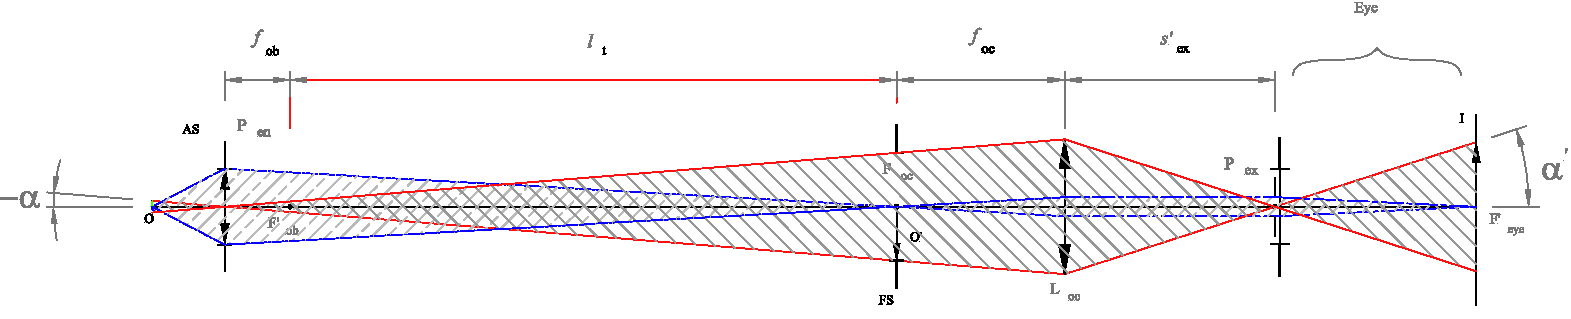
\includegraphics[width=\linewidth]{figs/microscopioEditado.pdf}
    \caption{Representación óptica del microscopio con un diafragma de apertura, la representación pupilas de entrada y salida y de los rayos marginal(azul) y principal (rojo). imagen obtenida de \cite{Yobani_Optica2020} y editada posteriormente}
    \label{fig:microscopio}
\end{figure}

A partir del comportamiento esperado en un microscopio, las pupilas de entrada se localiza en el lente OB, siendo este donde se ubica el diafragma de apertura de diámetro $D_{DA}$ que controla el cono de energía de entrada

(TABLA DE PUPILA SALIDA)
\begin{table}[H]
    \centering
    \begin{tabular}{c}
    \hline
        pupila salida \\ \hline 
            99.0 \\
            98.3\\
            99.1\\
            98.8\\
            98.5\\
            99.5\\
    \end{tabular}
    \caption{pupila salida}
    \label{tab:pupila_salida}
\end{table}

\begin{table}[H]
    \centering
    \begin{tabular}{c}
    \hline
        tamaño pupila \\ \hline 
            1.10    \\
            0.95    \\
            1.00    \\
            1.00    \\
            0.95    \\
            0.90    \\
    \end{tabular}
    \caption{tamaño}
    \label{tab:tamaño_pupila}
\end{table}

%==============================
% first problem
\begin{problem}{Posiciones de diafragmas}{diafragmas}

¿Cuáles son las posiciones adecuadas para colocar los diafragmas de apertura y de campo en el microscopio?

\end{problem}

\textbf{Diafragma de apertura}
Como se observa en la figura $\ref{fig:microscopio}$ las posición adecuada para colocar el diafragma de apertura es en el lente objetivo, pues como incialmente el diafragma de apertura es la lente objetivo, cuya imagen se forma en la pupila de salida, si se coloca un diafragma de apertura en un lugar diferente a la lente objetivo, la imagen del diafragma de apertura se forma en un lugar diferente, afectando la formación de la imagen final, pues la pupila del ojo debe coincidir con la pupila de salida para tener tanto mayor nitidez, como campo visual.

\textbf{Diafragma de campo}

Como se puede observar nuevamente en la figura $\ref{fig:microscopio}$, la posición adecuada para colocar el diafragma de campo es el foco primario del lente ocular, pues al ser este el lugar donde se forma la imagen producida por el lente objetivo, este diafragma de campo permite entonces controlar la porcion del objeto que se quiere visualizar, de forma tal que si se coloca un diafragma de campo menor que lente objetivo y la lente ocular, se vera necesariemente una menor porción del objeto, y si se coloca un diafragma de campo mayor, se vera una mayor porción del objeto, pero limitanda por la menor (en dimetro) de las dos lentes. Note que una ubicaicón diferente del diafragma de campo afectaria el control sobre el campo visual de la imagen.

%==============================
% fourth problem

\begin{problem}{Telescopio}{telescopio}

En la configuración del telescopio de la práctica, ¿cómo estimo el aumento? ¿Cuál es el aumento nominal de un telescopio refractor astronómico?

\end{problem}

%==============================
% Fifth problem



\begin{center}
\renewcommand{\arraystretch}{1.8}
\setlength{\tabcolsep}{8pt}
\begin{tabular}{|c|c|c|c|c|c|c|}
\hline
\parbox[c][5em][c]{2cm}{\centering \textbf{u} \\ $2.2\,\text{MeV}$ \\ $+\frac{2}{3}$ \\ $1/2$} &
\parbox[c][5em][c]{2cm}{\centering \textbf{d} \\ $4.7\,\text{MeV}$ \\ $-\frac{1}{3}$ \\ $1/2$} &
\parbox[c][5em][c]{2cm}{\centering \textbf{$\bar{u}$} \\ $2.2\,\text{MeV}$ \\ $-\frac{2}{3}$ \\ $1/2$} &
\parbox[c][5em][c]{2cm}{\centering \textbf{$\bar{d}$} \\ $4.7\,\text{MeV}$ \\ $+\frac{1}{3}$ \\ $1/2$} &
\parbox[c][5em][c]{2cm}{\centering \textbf{e$^-$} \\ $0.511\,\text{MeV}$ \\ $-1$ \\ $1/2$} &
\parbox[c][5em][c]{2cm}{\centering \textbf{$\gamma$} \\ $0$ \\ $0$ \\ $1$} &
\parbox[c][5em][c]{2cm}{\centering \textbf{W$^+$} \\ $80.39\,\text{GeV}$ \\ $+1$ \\ $1$} \\ \hline

\parbox[c][5em][c]{2cm}{\centering \textbf{c} \\ $1.27\,\text{GeV}$ \\ $+\frac{2}{3}$ \\ $1/2$} &
\parbox[c][5em][c]{2cm}{\centering \textbf{s} \\ $96\,\text{MeV}$ \\ $-\frac{1}{3}$ \\ $1/2$} &
\parbox[c][5em][c]{2cm}{\centering \textbf{$\bar{c}$} \\ $1.27\,\text{GeV}$ \\ $-\frac{2}{3}$ \\ $1/2$} &
\parbox[c][5em][c]{2cm}{\centering \textbf{$\bar{s}$} \\ $96\,\text{MeV}$ \\ $+\frac{1}{3}$ \\ $1/2$} &
\parbox[c][5em][c]{2cm}{\centering \textbf{$\nu_e$} \\ $<2\,\text{eV}$ \\ $0$ \\ $1/2$} &
\parbox[c][5em][c]{2cm}{\centering \textbf{W$^-$} \\ $80.39\,\text{GeV}$ \\ $-1$ \\ $1$} &
\parbox[c][5em][c]{2cm}{\centering \textbf{Z$^0$} \\ $91.19\,\text{GeV}$ \\ $0$ \\ $1$} \\ \hline

\parbox[c][5em][c]{2cm}{\centering \textbf{t} \\ $172.76\,\text{GeV}$ \\ $+\frac{2}{3}$ \\ $1/2$} &
\parbox[c][5em][c]{2cm}{\centering \textbf{b} \\ $4.18\,\text{GeV}$ \\ $-\frac{1}{3}$ \\ $1/2$} &
\parbox[c][5em][c]{2cm}{\centering \textbf{$\bar{t}$} \\ $172.76\,\text{GeV}$ \\ $-\frac{2}{3}$ \\ $1/2$} &
\parbox[c][5em][c]{2cm}{\centering \textbf{$\bar{b}$} \\ $4.18\,\text{GeV}$ \\ $+\frac{1}{3}$ \\ $1/2$} &
\parbox[c][5em][c]{2cm}{\centering \textbf{$\mu^-$} \\ $105.66\,\text{MeV}$ \\ $-1$ \\ $1/2$} &
\parbox[c][5em][c]{2cm}{\centering \textbf{$\nu_\mu$} \\ $<0.17\,\text{MeV}$ \\ $0$ \\ $1/2$} &
\parbox[c][5em][c]{2cm}{\centering \textbf{$\tau^-$} \\ $1776.86\,\text{MeV}$ \\ $-1$ \\ $1/2$}\\ \hline

\parbox[c][5em][c]{2cm}{\centering \textbf{$\nu_\tau$} \\ $<0.018\,\text{MeV}$ \\ $0$ \\ $1/2$} &
\parbox[c][5em][c]{2cm}{\centering \textbf{$\bar{\tau}$} \\ $1776.86\,\text{MeV}$ \\ $+1$ \\ $1/2$} &
\parbox[c][5em][c]{2cm}{\centering \textbf{$\bar{e}$} \\ $0.511\,\text{MeV}$ \\ $+1$ \\ $1/2$} &
\parbox[c][5em][c]{2cm}{\centering \textbf{$\bar{\mu}$} \\ $105.66\,\text{MeV}$ \\ $+1$ \\ $1/2$} &
\end{tabular}
\end{center}



\begin{problem}{Conclusiones}{conclusiones}

En un párrafo, escriba sus conclusiones acerca del experimento.

\end{problem}

I use the package \texttt{physics} which provides a great variety of commands for common operations and symbols. For instance, instead of typing \verb|\dfrac{\partial x}{\partial t}|, the \texttt{physics} package provides the command \verb|\pdv{x}{t}| which gives the same result. I also defined my own commands, so you can take a look in the \texttt{commands.tex} file if you like. I'd also suggest to create a folder and work each problem in a separate \texttt{.tex} file. I already included such folder in the \texttt{Overleaf} template, but you won't see it if you download the \texttt{Github} template. 

% =================================================

% \newpage

% \vfill

\bibliographystyle{apalike}
\bibliography{references}

\end{document}